% Springer Nature journal article template (Version 3.1, December 2024)
% Compile with pdfLaTeX and BibTeX in a project containing sn-jnl.cls and
% sn-basic.bst from the official Springer Nature LaTeX template package.
\documentclass[pdflatex,sn-basic,Numbered]{sn-jnl}

\usepackage{graphicx}
\usepackage{amsmath,amssymb,amsfonts}
\usepackage{booktabs}
\usepackage{braket}
\usepackage{array}
\usepackage{tabularx}
\usepackage{enumitem}
\usepackage{seqsplit}
\usepackage[title]{appendix}

\newcommand{\ttf}[1]{\texttt{\seqsplit{#1}}}
\newcommand{\cx}[2]{CX($#1\!\to\!#2$)}
\newcommand{\snrest}{\mathrm{SNR}_{\mathrm{est}}}
\newcommand{\snrexact}{\mathrm{SNR}_{\mathrm{exact}}}
\newcommand{\vshots}{\mathrm{Var}_{\mathrm{shots}}}

\setlist{nosep,leftmargin=*}
\setlength{\emergencystretch}{1.5em}
\raggedbottom

\begin{document}

\title[Interaction-Aware Evaluation of QNN Trainability Strategies]
{Interaction-Aware Evaluation of Exact and Finite-Shot Gradient Resolvability in a Four-Qubit Hybrid Quantum Neural Network}

\author*[1]{\fnm{Brandon} \sur{Shen} \space(ORCID: \href{https://orcid.org/0009-0002-3545-2106}{0009-0002-3545-2106})} \email{brandonshen123@gmail.com}

\affil*[1]{\orgname{Carlmont High School},
\orgaddress{\street{1400 Alameda de las Pulgas}, \city{Belmont},
\state{California}, \postcode{94002}, \country{United States}}}


\abstract{\textbf{Purpose:} Trainability interventions for quantum neural networks are usually evaluated one at a time, even though architecture, objective choice, and hybrid connectivity can jointly determine whether a finite-shot gradient is usable. This study tests whether restricted entanglement, a local transverse-field-Ising-model energy objective, and a residual shortcut reinforce, duplicate, or interfere with one another.

\textbf{Methods:} All eight configurations of the three binary strategies are evaluated in a four-qubit measure--re-encode--reset hybrid quantum neural network across matched block-count and shot-budget sweeps. Outcomes include exact-gradient magnitude, end-to-end estimator signal-to-noise ratio (SNR), bias, sign agreement, task metrics, and measurement cost. Confirmatory mixed-effects models use Holm correction, supplemented by matched bootstraps, finite-difference validation, and sensitivity analyses.

\textbf{Results:} Restricted entanglement and the local objective show a positive interaction for exact-gradient magnitude ($\eta_{EL} = 0.0043$, $p_{\text{Holm}} = 0.013$), corroborated by a matched bootstrap. The corresponding end-to-end estimator-SNR interaction is positive under Wald/Holm inference ($\beta_{EL} = 0.025$, $p_{\text{Holm}} = 0.002$) but is not corroborated by an extended bootstrap and is operationally modest (a 3.4\% multiplicative SNR shift). No $E \times R$ interaction is detected, and the $L \times R \times$ block-count interaction is not rejected but is sensitive to estimator mode and depth range. Combining all three strategies does not consistently outperform the best single strategy.

\textbf{Conclusion:} Interaction-aware evaluation reveals composition effects that isolated ablations can miss. In this four-qubit noiseless case study, the positive exact-gradient $E \times L$ interaction is the most robust finding, while the analogous finite-shot evidence remains inference-method dependent.}

\keywords{quantum machine learning, quantum neural networks, factorial evaluation, finite-shot estimation, trainability, reproducible benchmarking}

\maketitle

\section{Introduction}\label{sec:introduction}

Variational quantum algorithms and quantum neural networks (QNNs) optimize parameterized quantum circuits through a classical feedback loop driven by measured expectation values or their derivatives \cite{cerezo2021vqa,mitarai2018quantum,schuld2019evaluating}. Their practical trainability depends on several coupled design choices: the circuit's expressive structure, the input state, the support and spectrum of the measured objective, parameter initialization, the optimizer, and the measurement protocol. Barren plateaus---regions in which gradients concentrate exponentially near zero with increasing problem size---are a central manifestation of this difficulty \cite{mcclean2018barren,holmes2022expressibility,larocca2025barren}. They are not, however, synonymous with trainability. Shallow models without asymptotic barren plateaus can still be obstructed by unfavorable local structure, initialization sensitivity, dataset-induced concentration, or finite-sampling uncertainty \cite{anschuetz2022traps,thanasilp2023subtleties}. This distinction motivates the narrower operational question studied here: whether a gradient component is resolvable under a specified finite-shot protocol.

Prior mitigation work has targeted different parts of the training pipeline. Local objectives can avoid the exponential gradient suppression associated with global observables under specified depth assumptions \cite{cerezo2021costfunction}; limiting random entanglement or selecting architecture-specific causal structure can preserve larger gradients \cite{ortizmarrero2021entanglement,patti2021entanglement,pesah2021qcnn}; and structured initialization or incremental circuit growth can delay entry into highly concentrated regions of parameter space \cite{grant2019identity,skolik2021layerwise}. Hybrid and dissipative QNN architectures introduce additional possibilities, but their trainability remains architecture dependent rather than automatic \cite{beer2020training,sharma2022dissipative}. Residual quantum networks provide a further architectural intervention and have shown improved optimization trajectories in specific QNN benchmarks \cite{kashif2024resqnets}.

Finite-shot implementation adds a second layer to the problem. Parameter-shift rules provide exact derivatives in the infinite-sampling limit for appropriate gates \cite{mitarai2018quantum,schuld2019evaluating}, but practical gradient estimates are stochastic and can require substantial measurement resources \cite{sweke2020stochastic}. Adaptive-shot optimizers explicitly allocate measurements according to estimated gradient uncertainty \cite{kubler2020adaptive,tamiya2022stochastic}; variance-reduction, circuit-structure, and backpropagation studies likewise show that gradient precision and acquisition cost depend on the model and observable being measured \cite{kreplin2024finite,chinzei2025tradeoff,bowles2025backpropagation}. Exact-gradient magnitude alone therefore does not determine whether an optimizer receives a reliable update direction.

These literatures establish that architecture, entanglement, objective locality, hybrid connectivity, and measurement allocation can each affect gradients. Recent theory has begun to place several sources of barren plateaus within unified algebraic descriptions rather than treating them as independent phenomena \cite{ragone2024lie}. Empirical mitigation studies nevertheless still tend to compare one intervention with one baseline. Such designs estimate marginal effects but cannot determine whether two interventions reinforce one another, duplicate the same mechanism, or interfere when combined. A complete factorial design estimates those interaction effects directly \cite{montgomery2019design}.

A prior companion review introduced pointwise finite-shot gradient SNR as an operational diagnostic for the 2--10-qubit regime and specified a complete $2^3$ factorial experiment crossing restricted entanglement, a local objective, and a residual shortcut \cite{shen2026gradient}. The review was conceptual: it defined the factors, directional prior, hypotheses, and analysis plan but contained none of the simulations or empirical results reported here. It underwent independent peer review and carries its own DOI and publication date, giving the prespecification claims made throughout the present manuscript (Section~\ref{sec:provenance}) an external, citable reference point rather than resting solely on the present author's own account. The present manuscript executes that design on ground-state preparation for a four-qubit open-boundary transverse-field Ising model (TFIM), using matched initializations, parameter identities, block counts, and total shot budgets. The primary finite-shot estimator re-estimates intermediate features within every replicate, representing the complete update signal supplied to an optimizer rather than an isolated node-level Jacobian estimate.

The study also includes an independent implementation and inference audit. The audit validates assembled hybrid gradients by black-box finite differences, examines the architecture's reset semantics and residual activation boundary, separates confirmatory and diagnostic estimator modes, assesses model and bootstrap stability, and records post-run amendments explicitly. This emphasis is substantive: in a finite-sample computational experiment, data-mode filtering, seed management, resource accounting, and regression tests determine which estimand is actually analyzed. Appendix~\ref{app:verification} summarizes the audit; full implementation-level detail (memory management, concurrency, and script-level provenance) is kept in the reproducibility index (Table~\ref{tab:repro-index}) and the archived verification records in the code repository rather than in the main narrative.

The contributions are fourfold:
\begin{enumerate}
\item We provide a complete factorial evaluation of three QNN gradient-resolvability strategies under matched initialization, parameter, architecture, and total-shot conditions.
\item We separate exact-gradient magnitude, estimator SNR, bias, sign agreement, task metrics, and measurement cost rather than treating any single quantity as a complete measure of trainability.
\item We release a reproducible implementation with deterministic seed derivation, finite-difference gradient validation, guarded estimator-mode separation, frozen result files, and regression tests covering the principal analysis paths.
\item In the four-qubit case study, we identify a robust positive interaction between restricted entanglement and the TFIM-energy objective at the exact-gradient level. The corresponding finite-shot interaction is directionally consistent but inference-method dependent, and combining all three interventions does not consistently outperform the best single intervention.
\end{enumerate}

\section{Related Work and Confirmatory Questions}

\subsection{From barren plateaus to finite-sample gradient usability}

A barren plateau is conventionally defined through asymptotic concentration of a loss or its derivatives as the number of qubits grows \cite{mcclean2018barren,larocca2025barren}. For a gradient component,
\[
\mathrm{Var}[\partial_\theta C] \in O(b^{-n}), \qquad b>1.
\]
The phenomenon can arise from excessive expressibility, global observables, entanglement structure, unfavorable data encoding, or hardware noise \cite{cerezo2021costfunction,ortizmarrero2021entanglement,wang2021noise,thanasilp2023subtleties,ragone2024lie}. Architecture-specific results also show that some structured models avoid exponential gradient suppression under their stated assumptions \cite{pesah2021qcnn}, whereas dissipative or reset-based architectures are not uniformly protected \cite{sharma2022dissipative}.

The present experiment does not estimate an asymptotic scaling class. A four-qubit block-count sweep cannot establish whether a gradient variance decays exponentially or polynomially with qubit number. Moreover, the absence of a barren plateau is not sufficient for successful optimization: shallow local models can still exhibit poor local minima or require impractically many noisy queries \cite{anschuetz2022traps}. We therefore use exact-gradient landscape statistics as theoretical diagnostics while asking a finite-sample question at fixed parameter points: is the update signal distinguishable from its repeated-shot uncertainty?

For parameter $\theta_k$, let $\hat g_k(\theta)$ be the complete finite-shot gradient estimator and $\mu_k(\theta)=\mathbb{E}_{\mathrm{shots}}[\hat g_k(\theta)]$ its repeated-shot mean at fixed $\theta$. The primary operational metric is
\[
\snrest(\theta)=
\frac{|\mu_k(\theta)|}
{\sqrt{\vshots[\hat g_k(\theta)\mid\theta]}}.
\]
When an exact statevector derivative is available, the complementary resolvability measure is
\[
\snrexact(\theta)=
\frac{|g_k^{\mathrm{exact}}(\theta)|}
{\sqrt{\vshots[\hat g_k(\theta)\mid\theta]}},
\]
and estimator bias is
\[
\mathrm{Bias}_k(\theta)=
\mu_k(\theta)-g_k^{\mathrm{exact}}(\theta).
\]
High $\snrest$ means that the estimator's own mean is resolvable under the stated protocol; it does not establish unbiasedness, correct sign, convergence, or task fidelity. Accordingly, $\snrexact$, bias, sign agreement, exact-gradient landscape variance, energy, and global fidelity are reported separately.

SNR-like precision criteria are already embedded in adaptive-shot optimization, where the number of measurements is adjusted according to estimated gradient means and variances \cite{kubler2020adaptive,tamiya2022stochastic}. Finite-sampling noise can also be reduced through objective regularization or more efficient gradient-acquisition schemes \cite{kreplin2024finite,chinzei2025tradeoff,bowles2025backpropagation,qiu2026tilted}. The novelty tested here is therefore not the ratio itself. It is the use of pointwise estimator SNR, exact references, bias diagnostics, and matched resource accounting as a common outcome framework for estimating interactions among multiple mitigation strategies.

\subsection{Mitigation strategies and possible interactions}

\textbf{Restricted entanglement ($E$).} Expressibility and entanglement are closely linked to gradient concentration. Highly expressive random circuits approach unitary designs and develop small gradients \cite{mcclean2018barren,holmes2022expressibility}, while entanglement growth has been identified as a direct contributor to barren plateaus \cite{ortizmarrero2021entanglement}. Entanglement-aware mitigation proposals consequently restrict connectivity, regularize entanglement, partition registers, or otherwise reduce random correlation spreading \cite{patti2021entanglement}. The factor used here changes the within-block CNOT schedule while holding the number of rotations and logical CNOT gates fixed. It is therefore a controlled architectural restriction, not a claim that low entanglement is universally optimal.

\textbf{Local objective ($L$).} Cost-function support can determine gradient scaling. For shallow alternating-layer ansätze that satisfy the assumptions of Cerezo et al., global observables produce exponentially vanishing gradients, whereas local observables yield at worst polynomial decay over a logarithmic-depth regime \cite{cerezo2021costfunction}. The present local factor replaces global target-state infidelity with normalized TFIM energy. Because these objectives differ in spectral weighting, observable decomposition, and measurement requirements as well as locality, the factor should be interpreted as the full objective contrast rather than as a pure locality intervention.

\textbf{Residual shortcut ($R$).} Residual connections can preserve information pathways and have improved training behavior in the ResQNet architecture \cite{kashif2024resqnets}. Related work on deep and dissipative QNNs shows, however, that reset, pooling, and ancilla-mediated architectures have trainability properties tied to their exact causal structure \cite{beer2020training,sharma2022dissipative,pesah2021qcnn}. The residual factor here is a fixed-gain classical shortcut between independently reset quantum blocks. It adds no quantum gates or observables and is narrower than the broader class of residual quantum architectures.

Initialization, parameter correlation, and layerwise growth provide additional mitigation families not crossed in this experiment \cite{grant2019identity,skolik2021layerwise}. Their exclusion is deliberate: the goal is not an exhaustive benchmark of all known strategies, but a factorial test of three interventions that act at different points in the hybrid computation---within-block entangling structure, objective construction, and between-block classical connectivity.

\subsection{Interaction gap and mechanistic expectation}

Theoretical work increasingly emphasizes that expressibility, state structure, observables, and noise should not be understood as independent sources of trainability behavior \cite{ragone2024lie}. Yet the empirical literature supporting the three interventions above evaluates them primarily in separate architectures and against separate baselines \cite{cerezo2021costfunction,ortizmarrero2021entanglement,patti2021entanglement,kashif2024resqnets}. We are not aware of a prior study that crosses these three specific interventions in a complete $2^3$ design under a common finite-shot gradient estimator. The novelty claim is correspondingly narrow: none of the individual interventions or metrics is new; the contribution is direct estimation of their pairwise and higher-order composition effects under matched conditions.

The strongest mechanistic expectation concerns $E\times L$. For a local objective written as a weighted sum of fixed observables,
\[
g^{\mathrm{exact}}_k(\theta)
=\sum_m w_m\,\mathrm{Tr}\!\left[
\frac{\partial\rho_{S_m}}{\partial\theta_k}L_{S_m}\right],
\]
a restricted entangling architecture changes the reduced-state derivatives, whereas the local objective selects and weights the derivative components entering the measured signal. Their effects can therefore overlap. The companion review treated sub-additivity as an interpretive prior at the exact-signal level, not as a theorem; all confirmatory interaction tests are two-sided \cite{shen2026gradient}. No directional prior was assigned to interactions involving the residual shortcut.

\subsection{Confirmatory hypotheses}

H1--H4 form one Holm-corrected family at family-wise $\alpha=0.05$:

\begin{itemize}
\item \textbf{H1, exact signal:} Is the $E\times L$ coefficient $\eta_{EL}$ in a mixed model of $\operatorname{asinh}(|g^{\mathrm{exact}}|)$ distinguishable from zero?
\item \textbf{H2, estimator SNR:} Is the $E\times L$ coefficient $\beta_{EL}$ in the end-to-end estimator-SNR model distinguishable from zero?
\item \textbf{H3, estimator SNR:} Is the $E\times R$ coefficient $\beta_{ER}$ distinguishable from zero?
\item \textbf{H4, block-count moderation:} Is the $L\times R\times\text{block-count}$ coefficient $\beta_{LRd}$ distinguishable from zero?
\end{itemize}

The three-way interaction, conditional-estimator analyses, checkpoint analyses, active-residual subset analyses, and comparisons between the fully combined condition and the best single intervention are not members of the confirmatory family.

\section{Evaluation Protocol and Experimental Setup}\label{sec:methods}

\subsection{Reference task and objectives}

The reference task is ground-state preparation for the four-site, open-boundary TFIM,
\[
H=-J\sum_{i=0}^{2}Z_i Z_{i+1}-h\sum_{i=0}^{3}X_i,
\qquad J=1,\quad h=0.5.
\]
The target ground state $\ket{\psi_0}$ and eigenvalue bounds $E_0\approx-3.4270$ and $E_{\max}\approx3.4270$ are obtained by exact diagonalization of the $16\times16$ Hamiltonian matrix. Let $\rho_0=\ket{\psi_0}\!\bra{\psi_0}$ and let $\rho(\theta)$ be the prepared state. The global objective is target-state infidelity,
\[
C_{\mathrm{global}}(\theta)
=1-\mathrm{Tr}[\rho_0\rho(\theta)],
\]
and the local objective is normalized TFIM energy,
\[
C_{\mathrm{local}}(\theta)
=\frac{\mathrm{Tr}[H\rho(\theta)]-E_0}{E_{\max}-E_0}.
\]
Both objectives have the same nondegenerate target ground state, preventing target identity from confounding the comparison. The resulting factor still represents the full contrast between normalized TFIM energy and global infidelity, not measurement locality alone: the objectives also differ in spectral weighting, observable decomposition, measurement requirements, and landscape geometry. Final energy and global fidelity are therefore reported for every configuration regardless of which objective is optimized.

\subsection{Hybrid block architecture and entangling schedules}
\label{sec:ansatz}

To avoid conflict with the local-cost factor $L$, the number of hybrid blocks is denoted by $D\in\{1,2,3,4,6\}$. Each block applies one independently parameterized $R_y$ rotation to each qubit, followed by exactly four logical CNOT gates. $D$ is a \emph{hybrid block count}, not the depth of one continuously evolving quantum state: each block is reset, evaluated, and measured independently, and later blocks receive only classically re-encoded features. The results therefore apply specifically to the measure--re-encode--reset architecture defined below.

Two logical CNOT schedules are used within each block:

\begin{itemize}
\item \textbf{Baseline ($E=0$):} \cx{0}{1}, \cx{1}{2}, \cx{2}{3}, \cx{3}{0}, in that order. The sequential schedule contains a causal path spanning the register within the block.
\item \textbf{Restricted ($E=1$):} odd-position blocks use \cx{0}{1}, \cx{2}{3}, \cx{1}{0}, \cx{3}{2}; even-position blocks use \cx{1}{2}, \cx{3}{0}, \cx{2}{1}, \cx{0}{3}. Each block acts within two disjoint pairs, with the pairing alternating by block position.
\end{itemize}

Both schedules are applied literally, gate by gate, in the statevector simulator, with no transpiler-level fusion or reordering. Because no quantum state persists across blocks, alternating the restricted schedule changes the paired qubits at each block position but does not accumulate entanglement across $D$ in the manner of alternating layers in one continuous circuit. Entanglement entropy and reduced-state purity are used only as finite-system diagnostics; no area-law or asymptotic scaling claim is made from four qubits.

\subsection{Residual hybrid architecture}
\label{sec:residual-arch}

For block $\ell\in\{1,\ldots,D\}$, the quantum node is
\[
z_j^{(\ell)}
=\mathrm{Tr}\!\left[Z_j\rho_\ell
  \!\left(x^{(\ell)},\theta^{(\ell)}\right)\right],
\qquad j=0,\ldots,3.
\]
The block is initialized from $\ket{0\ldots0}$ and depends only on its own encoded input $x^{(\ell)}$ and gate angles $\theta^{(\ell)}$. For $\ell=1,\ldots,D-1$, the next input is
\[
x^{(\ell+1)}=
\begin{cases}
W_\ell z^{(\ell)}+b_\ell+\gamma z^{(\ell-1)}, & R=1,\\[3pt]
W_\ell z^{(\ell)}+b_\ell, & R=0,
\end{cases}
\]
with fixed shortcut gain $\gamma=1$ in the residual condition and $\gamma=0$ otherwise. $W_\ell$ and $b_\ell$ are parameterized and initialized identically across residual and non-residual conditions; the fixed shortcut adds no trainable parameters, quantum gates, or additional observables.

The boundary convention is $z^{(0)}=0$. Therefore, the shortcut first changes a real block input at $x^{(3)}=W_2z^{(2)}+b_2+\gamma z^{(1)}$, which exists only when $D\ge3$. Thus, under matched seeds, $R=0$ and $R=1$ are structurally identical at $D\in\{1,2\}$ and diverge only from $D=3$ onward.

This activation threshold was identified during the post-run implementation audit, not in the companion review's prespecified H3/H4 analysis \cite{shen2026gradient}. It therefore does not retroactively redefine the confirmatory population. The original full-sweep models remain primary. A $D\ge3$ active-residual analysis is reported as a sensitivity analysis, and the exact zero residual contrast at $D\in\{1,2\}$ is reported as a structural-validity check.

\subsection{Gradient assembly and validation target}

The terminal block's gradient is a direct parameter-shift derivative of the final cost. Every upstream total derivative is assembled by reverse-mode chain rule through the classical maps and quantum-node Jacobians,
\[
\frac{dC}{d\theta_k^{(\ell)}}
=\sum_j
\frac{\partial C}{\partial z_j^{(\ell)}}
\frac{\partial z_j^{(\ell)}}{\partial\theta_k^{(\ell)}}.
\]
Node-level derivatives are evaluated by the two-term parameter-shift rule for Pauli-generated rotations \cite{mitarai2018quantum,schuld2019evaluating}; the downstream sensitivities are propagated exactly through the classical maps. Classical gradients with respect to $W_\ell$ and $b_\ell$ are analyzed separately and are not pooled into the matched quantum-gradient distribution.

The finite-difference audit treats the complete hybrid cost as a black box and compares central finite differences against the assembled total derivative. The audit design is described here; numerical outcomes are reported in Section~\ref{sec:results-robustness} and Appendix~\ref{app:verification}.

\subsection{Complete factorial design}

All combinations of $E,L,R\in\{0,1\}^{3}$ are run (Table~\ref{tab:configurations}).

\begin{table*}[t]
\centering
\begin{tabular}{cccc l}
\toprule
\# & $E$ & $L$ & $R$ & Description \\
\midrule
1 & 0 & 0 & 0 & Baseline \\
2 & 1 & 0 & 0 & Restricted entanglement only \\
3 & 0 & 1 & 0 & Local cost only \\
4 & 0 & 0 & 1 & Residual only \\
5 & 1 & 1 & 0 & $E+L$ (H1/H2 contrast) \\
6 & 1 & 0 & 1 & $E+R$ (H3 contrast) \\
7 & 0 & 1 & 1 & $L+R$ (H4 contrast) \\
8 & 1 & 1 & 1 & All three interventions \\
\bottomrule
\end{tabular}
\caption{Complete $2^3$ factorial design.}
\label{tab:configurations}
\end{table*}

Within each hybrid block count, all configurations share initialization seeds, matched quantum-gate parameter indices, and the same nominal shot-budget levels.

\subsection{Finite-shot estimator modes}

Two finite-shot modes are collected and reported separately:

\begin{itemize}
\item \textbf{End-to-end mode, confirmatory for H2--H4:} forward features and node-level shifted measurements are independently re-estimated in every replicate. Nonlinear downstream re-encoding can therefore induce finite-shot estimator bias.
\item \textbf{Conditional mode, diagnostic:} forward features are held at their exact statevector values while node-level shifted measurements are resampled. This isolates Jacobian-estimation noise from uncertainty caused by re-estimating and re-encoding intermediate features.
\end{itemize}

The conditional mode is not a second confirmatory test and cannot replace an unfavorable end-to-end result. Material disagreement between the modes is interpreted as sensitivity to forward-feature sampling rather than resolved by selecting the more favorable estimator.

For every configuration, block count, initialization, matched quantum-gate parameter, and budget level $B\in\{250,500,1000,2000\}$, $R_{\mathrm{rep}}$ independent gradient replicates are generated. Their mean, sampling variance, $\snrest$, $\snrexact$, bias, and sign agreement are computed pointwise before aggregation.

\subsection{Measurement-budget accounting}
\label{sec:budget}

The symbol $B$ denotes the total shot budget for one replicate's complete gradient vector. The implementation floor-divides $B$ across every required measurement job and distributes the remainder deterministically one shot at a time, so the realized total shot count equals $B$ in every cell. The global and local objectives nevertheless require different numbers of observable bases, and end-to-end mode adds forward-feature measurement jobs. Consequently, configurations compared at the same $B$ can receive different shots per circuit even though their total-shot budgets are exactly matched. The implementation records shifted circuits, forward-feature circuits, observable settings, total jobs, and shots per circuit. Confirmatory inference uses the prespecified $\log_2(B)$ factor; per-circuit precision and job-count differences are reported as resource diagnostics rather than treated as matched.

\subsection{Primary summaries and estimator-fidelity diagnostics}

The matched quantum-gradient distribution is summarized by the median and interquartile range of pointwise $\snrest$, the fraction of components with $\snrest\ge1$, and dependence on $D$ and $B$. The threshold one is descriptive only: it indicates that the estimator mean equals or exceeds one estimated sampling standard deviation and is not treated as a necessary or sufficient condition for optimization success.

Where exact derivatives are available, the analysis additionally reports $\snrexact$, signed and absolute bias, and
\[
\mathbb{1}\!\left[
\operatorname{sign}(\mu_k)
=\operatorname{sign}(g_k^{\mathrm{exact}})
\right].
\]
Exact-gradient landscape variance is calculated across matched initializations and remains distinct from repeated-shot variance at fixed parameters.

\subsection{Pilot-informed replicate and initialization counts}
\label{sec:calibration}

The independent pilot begins from $R_{\mathrm{rep}}=30$ replicates per cell and $N_{\mathrm{init}}=50$ matched initializations. Replicate count is increased until bootstrap interval widths for both the signed mean and $\snrest$ meet the prespecified precision criterion and stabilize across the next increment. Bootstrap resampling follows standard nonparametric principles \cite{davison1997bootstrap}; the criterion is motivated operationally by adaptive-shot work \cite{tamiya2022stochastic}. Because $\snrest$ is a plug-in ratio involving an estimated standard deviation, its own Monte Carlo uncertainty can remain large after the signed mean is already well resolved.

Candidate initialization counts are evaluated in increments of 25. The selected count is the smallest candidate for which the 90th percentile of the simulated 95\% confidence-interval half-width is at most 0.20 for every primary interaction coefficient. Actual convergence, failures to meet a criterion, and any recollection are Results items rather than assumed successes; the manuscript therefore uses \emph{pilot-informed}, not \emph{pilot-calibrated}, sample sizes.

\subsection{Analysis provenance and amendments}
\label{sec:provenance}

The companion review prespecified the eight configurations, the block-count and shot-budget sweeps, end-to-end estimator SNR as the primary finite-shot outcome, the two mixed-effects model families, H1--H4, the $\operatorname{asinh}$ transformations, and Holm correction \cite{shen2026gradient}. The following items were identified or modified during the subsequent audit and are not presented as prespecified confirmatory choices:

\begin{itemize}
\item recognition that $R$ is structurally inactive at $D\in\{1,2\}$;
\item the $D\ge3$ active-residual subset models;
\item finite-difference checks and any ad hoc depth-moderation refits;
\item computational redesign of the bootstrap implementation;
\item any additional model term, diagnostic, or resource-normalized outcome not listed in the companion review \cite{shen2026gradient}.
\end{itemize}

These analyses can validate implementation, explain heterogeneity, or test robustness, but they do not replace the original confirmatory estimands.

\subsection{Mixed-effects models}

Let $i$ index initialization, $c$ configuration, $p$ the matched quantum-gate parameter within a block count, $d$ block count, and $b$ shot budget. The three binary intervention indicators are effect coded as $\widetilde E_c,\widetilde L_c,\widetilde R_c\in\{-1/2,+1/2\}$, and $\widetilde D_d$ is block count centered and scaled to unit standard deviation. Effect coding makes lower-order coefficients average effects across the other factorial conditions. The matched repeated-measures structure is represented by a random intercept $u_i$ for initialization and a random intercept $v_{idp}$ for the matched parameter nested within initialization and block count. Mixed-effects estimation follows standard linear mixed-model practice \cite{bates2015lme4}.

For H1, the response is $a_{icpd}=\operatorname{asinh}(|g^{\mathrm{exact}}_{icpd}|)$. The model contains all intervention main effects, all pairwise products, the three-way product, centered block count, the three intervention-by-block-count terms, and the two random intercepts. The $E\times L$ coefficient is $\eta_{EL}$.

For H2--H4, the response is $y_{icpdb}=\operatorname{asinh}(\mathrm{SNR}_{\mathrm{est},icpdb})$, and $s_b=\log_2(B_b)$. The prespecified model is
\begin{align*}
y_{icpdb}={}&\beta_0
+\beta_E\widetilde E_c
+\beta_L\widetilde L_c
+\beta_R\widetilde R_c\\
&+\beta_{EL}\widetilde E_c\widetilde L_c
+\beta_{ER}\widetilde E_c\widetilde R_c
+\beta_{LR}\widetilde L_c\widetilde R_c\\
&+\beta_{ELR}\widetilde E_c\widetilde L_c\widetilde R_c
+\beta_D\widetilde D_d+\beta_B s_b\\
&+\beta_{ED}\widetilde E_c\widetilde D_d
+\beta_{LD}\widetilde L_c\widetilde D_d
+\beta_{RD}\widetilde R_c\widetilde D_d\\
&+\beta_{LRD}\widetilde L_c\widetilde R_c\widetilde D_d
+u_i+v_{idp}+\varepsilon_{icpdb}.
\end{align*}
H2 tests $\beta_{EL}=0$, H3 tests $\beta_{ER}=0$, and H4 tests $\beta_{LRD}=0$. The three-way coefficient is exploratory. The confirmatory model uses the full prespecified $D$ sweep. A separate $D\ge3$ fit reports the same residual-related coefficients as a post-run sensitivity analysis.

All mixed-effects models are fit in Python 3.12.10 with statsmodels 0.14.6, REML, and an L-BFGS-first optimizer fallback order (BFGS, CG, Powell, Nelder--Mead attempted only if L-BFGS fails to converge); no custom convergence tolerances are set beyond each optimizer's library default. A fit is flagged singular if either variance component is within $10^{-8}$ of zero. Every confirmatory and sensitivity fit in this paper converged and none was singular; an independent BFGS refit of the adopted H2--H4 model agrees with the default L-BFGS fit to 8--9 significant figures (Section~\ref{sec:results-robustness}). Full package versions, random-seed derivation, and bootstrap sharding are reported in the Software Availability and Reproducibility Information section below.

\subsection{Inference and multiplicity}

Primary coefficient tests use model-based Wald standard errors and two-sided $p$-values. H1--H4 form one family, corrected by the sequential Holm procedure at family-wise $\alpha=0.05$ \cite{holm1979sequential}. Effect estimates, unadjusted confidence intervals, raw $p$-values, and Holm-adjusted $p$-values are all reported; a confirmatory rejection requires the adjusted criterion. Failure to reject is not interpreted as equivalence without a prespecified smallest effect of interest and an equivalence test.

A nested matched bootstrap propagates finite-$R_{\mathrm{rep}}$ uncertainty into coefficient intervals \cite{davison1997bootstrap}. Outer resampling is by complete matched initialization, retaining all eight configurations, block counts, budgets, and parameter identities. Within each selected initialization--configuration--parameter--block-count--budget cell, gradient replicates are resampled; the pointwise mean, variance, and SNR are recomputed; and the full model is refit. Achieved iteration counts and Monte Carlo stability are reported rather than assumed.

\subsection{Secondary interaction indices}

For strategies $A$ and $B$, let $M_A$ denote RMS pointwise $\snrest$ and $G_A$ RMS exact-gradient magnitude over the same matched points. Secondary multiplicative indices are
\[
I_{AB}=\frac{M_{AB}M_0}{M_A M_B},
\qquad
J_{AB}=\frac{G_{AB}G_0}{G_A G_B}.
\]
Values below, equal to, or above one indicate sub-additive, multiplicatively independent, or super-additive fold changes on this selected scale. These indices do not replace the factorial regression, are undefined when a required aggregate is zero, and are accompanied by medians, interquartile ranges, matched distributions, and additive-scale sensitivity analyses.

\subsection{Independent implementation and inference audit}
\label{sec:implementation-notes}

The audit had four components: (1) black-box central finite differences on the complete hybrid cost; (2) inspection of reset-versus-state-carryover block semantics; (3) independent checks of the residual activation boundary; and (4) regression testing of the memory-efficient bootstrap against the original implementation on identical resamples. Procedures are described here; quantitative outcomes and any unresolved limitations are reported in Section~\ref{sec:results-robustness} and Appendix~\ref{app:verification}.

\subsection{Use of large language models}

OpenAI ChatGPT was used during 2026 to support literature-search planning, clarification of technical concepts, implementation and verification scripting, and feedback on author-written prose. The tool was not treated as an author or as an evidentiary source. The author independently inspected the primary literature, executed and reviewed the code, verified numerical outputs, and accepts responsibility for every claim, citation, analysis decision, and final wording in this manuscript.

\section{Results}

\subsection{Calibration outcomes}
\label{sec:results-calibration}

$N_{\mathrm{init}}$ converged cleanly at its floor candidate, $N_{\mathrm{init}}=50$: simulated 90th-percentile 95\% CI half-widths for the three primary interaction coefficients were $0.103$, $0.103$, and $0.073$, each under the prespecified $0.20$ target, so no larger candidate was needed.

$R_{\mathrm{rep}}$ did \emph{not} converge uniformly. At the committed $R_{\mathrm{rep}}=30$, the rate of pointwise cells with exactly zero replicate variance (excluded from the SNR model, not imputed) ran from $4.4\%$ at block count $1$/budget $250$ down to $1.3\%$ at block count $1$/budget $2000$, versus $0.1$--$1.1\%$ at every deeper block count. Raising the calibration ceiling to $R_{\mathrm{rep}}=500$ for the four worst-affected block-count-1 pilot cells resolved only one of them (at $R_{\mathrm{rep}}=270$); the other three did not converge even at $500$, with one extrapolated to require roughly $170\times$ the committed value. Non-convergence was consistently worse at higher nominal shot budget within the same cell---a signature of $\mathrm{SNR}_{\mathrm{est}}$'s own plug-in-ratio sampling distribution being harder to resolve as per-replicate noise shrinks, not evidence that the underlying gradient measurements became noisier. Recollecting the affected cells at $R_{\mathrm{rep}}\approx270$--$300$ was found to be cheap (minutes), but was not done for the confirmatory dataset reported below; block-count-1 estimates should accordingly be read as carrying wider uncertainty than deeper block counts. Because zero estimated variance may be associated with specific configurations rather than missing completely at random, inference is conditional on this exclusion rule.

\subsection{Zero-variance exclusion and block-count sensitivity}
\label{sec:zero-variance-sensitivity}

Two post-run robustness checks address the zero-variance exclusion rule introduced in Section~\ref{sec:results-calibration}: a $D=1$-exclusion refit of the H2--H4 model, and a full tabulation of where zero-variance exclusions occur. Both are post-run, data-dependent checks, not part of the prespecified confirmatory family, and neither replaces the full-sweep confirmatory H2--H4 model or the existing $D\ge3$ active-residual sensitivity fit (Section~\ref{sec:residual-arch}), which is a distinct, more aggressive exclusion (it additionally drops $D=2$).

\textbf{$D=1$-exclusion sensitivity.} Refitting H2--H4 on $D\in\{2,3,4,6\}$ (excluding $D=1$ entirely, end-to-end mode, identical formula, coding, and $\widetilde D$ scaling to the full-sweep fit) gives:

\begin{itemize}
\item $\beta_{EL}$: $0.024996\to0.032354$ (SE $0.007279\to0.007087$, $p=0.000595\to4.99\times10^{-6}$), a shift of $+1.011$ original-standard-error units. The sign agrees and the Wald confidence intervals overlap extensively ($[0.010729,0.039263]$ vs.\ $[0.018464,0.046244]$).
\item $\beta_{ER}$: $-0.000958\to-0.000941$, a shift of $+0.002$ original-SE units---sign agrees, intervals overlap almost completely.
\item $\beta_{LRd}$: $-0.010179\to-0.009847$, a shift of $+0.062$ original-SE units---sign agrees, intervals overlap extensively.
\end{itemize}

$\beta_{ER}$ and $\beta_{LRd}$ show little sensitivity to excluding $D=1$. $\beta_{EL}$'s movement is flagged rather than dismissed: the estimate remains positive and becomes \emph{more} statistically separated from zero after removing $D=1$ (not less), which is inconsistent with $D=1$ alone generating the positive interaction---if $D=1$ were driving a spurious super-additive signal, removing it would be expected to shrink the estimate toward zero or widen its interval, not sharpen it. This pattern does not, however, explain \emph{why} the point estimate itself moves by approximately one original standard error under this specific exclusion; it is reported as a sensitivity of the estimated magnitude and precision to the depth range analyzed, not as proof that the movement is scientifically inconsequential.

\textbf{Zero-variance exclusion audit.} Tabulating every pointwise cell excluded for exactly zero estimated replicate variance (the rule introduced in Section~\ref{sec:results-calibration}; no epsilon was added, and no excluded cell was imputed or regularized) reveals a pattern more extensive than a block-count-1 effect alone: \textbf{zero-variance exclusion is exactly confined to $L=0$} cells, in both the end-to-end and conditional estimator modes, across the complete depth and budget design. None of the 102,400 $L=1$ cells in either mode is ever excluded; all 1,833 excluded cells (509 end-to-end, 1,324 conditional) come from the 102,400 $L=0$ cells in each mode. The exclusion rate is highest at $D=1$ in end-to-end mode ($2.58\%$) but is not a $D=1$-specific phenomenon: it persists at every deeper block count ($D=2$ through $D=6$, approximately $0.27\%$--$0.66\%$), always confined to $L=0$.

This is stated plainly because $L$ is one of the two factors in the paper's headline $E\times L$ interaction: the confirmatory estimator-SNR analysis is therefore conditional on an eligibility/exclusion process that is perfectly associated with cost type, not merely more common at low block count. The analysis documents this selection pattern but does not establish its physical or computational mechanism---no forced explanation is offered, and no claim is made that $L=1$ is a "better" condition merely because it produced no exactly-zero replicate-variance cells. An exploratory logistic model, $\text{zero-variance excluded}\sim E*L*R+\log_2(B)$, was attempted at $D=1$ and exhibited complete quasi-separation on $L$ (a mechanical consequence of $L=1$ contributing zero events in every stratum); no coefficient from that model is reported, and the descriptive tabulation above is presented as the defensible result instead.

Figure~\ref{fig:d1-sensitivity} shows the full-sweep and $D\neq1$ Wald intervals for all three H2--H4 coefficients; Figure~\ref{fig:zero-variance-heatmap} shows the end-to-end, $D=1$ exclusion-rate heatmap by configuration and budget, the stratum in which the pattern above is most visible.

\begin{figure}[t]
\centering
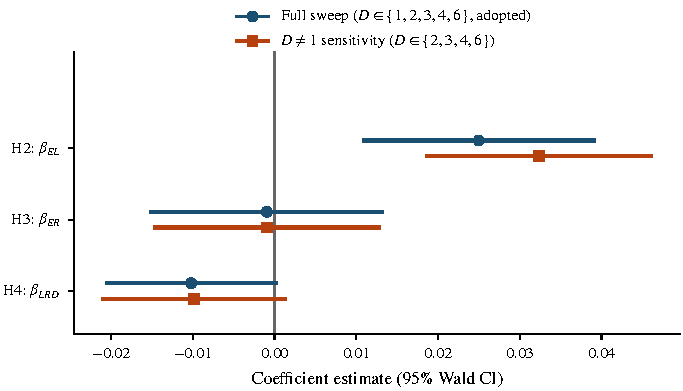
\includegraphics[width=\columnwidth]{figures/fig6_d1_exclusion_sensitivity.pdf}
\caption{Adopted full-sweep ($D\in\{1,2,3,4,6\}$) and $D\neq1$-sensitivity
($D\in\{2,3,4,6\}$) H2--H4 estimates with 95\% Wald confidence intervals.
The $D\neq1$ model is a sensitivity analysis, not a replacement for the
full-sweep confirmatory model; $\beta_{EL}$ moves further from zero and
$\beta_{ER}$/$\beta_{LRd}$ are comparatively stable under this exclusion.}
\label{fig:d1-sensitivity}
\end{figure}

\begin{figure}[t]
\centering
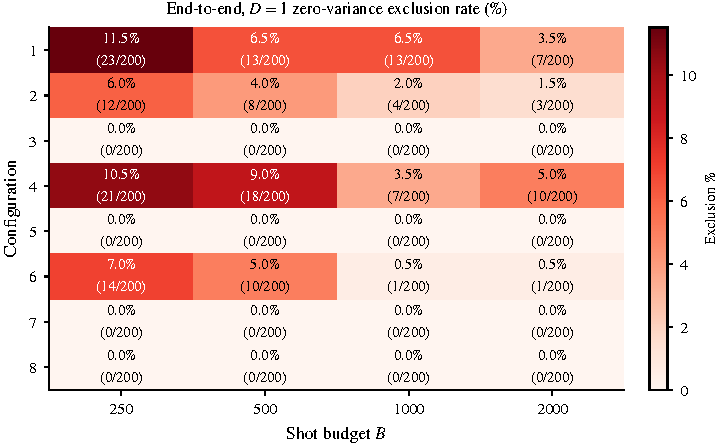
\includegraphics[width=\columnwidth]{figures/fig7_zero_variance_exclusion_rates.pdf}
\caption{End-to-end, $D=1$ zero-variance exclusion percentage by
configuration and shot budget $B$, with raw excluded/total counts
annotated. This is a descriptive exclusion-rate tabulation, not a measure
of gradient magnitude or estimator SNR; every nonzero cell in this figure
has $L=0$, and every $L=1$ configuration (3, 5, 7, 8) shows exactly $0\%$
at every budget. The pattern is descriptive of the selection process
underlying the confirmatory model, not a causal claim about its mechanism.}
\label{fig:zero-variance-heatmap}
\end{figure}

\subsection{\texorpdfstring{H1---exact-signal $E\times L$ interaction ($\eta_{EL}$)}{H1---exact-signal E x L interaction}}

$\eta_{EL}=0.004346$ (SE $0.001529$, Wald $z=2.84$), $p=0.00448$, $p_{\mathrm{Holm}}=0.0134$: \textbf{rejected}. The interaction is \textbf{super-additive} (positive)---the opposite direction from the companion review's one prespecified interpretive expectation (sub-additivity at the exact-signal level) \cite{shen2026gradient}. This is reported as a direct contradiction of that prior, not reframed to fit it.

Two independent checks rule out an implementation artifact. First, black-box finite differences on the full multi-block hybrid cost agree with the assembled gradient to a worst relative error of $1.27\times10^{-5}$ overall ($9.77\times10^{-7}$ among non-floor-dominated components), with clean $O(h^2)$ truncation convergence before the expected floating-point floor (Appendix~\ref{app:verification}, A.1). Second, an apparent block-count-1-versus-6 sign reversal in a small subsample was traced to small-sample noise: an ad hoc $E{:}L{:}\widetilde D$ term added to the exact-signal model and fit on the full $25{,}600$-row exact dataset gives $E{:}L=+0.003805$ and $E{:}L{:}\widetilde D=+0.001005$ (SE $0.001125$, not distinguishable from zero)---the super-additive direction is essentially block-count-invariant, not an artifact of pooling over a range that secretly disagrees with itself.

A nested bootstrap at $n=400$ iterations gives a percentile interval $[0.000810, 0.008027]$, excluding zero in the same direction as the Wald result---the first non-Wald corroboration obtained anywhere in this study.

\subsection{\texorpdfstring{H2---end-to-end estimator-SNR $E\times L$ interaction ($\beta_{EL}$)}{H2---end-to-end estimator-SNR E x L interaction}}

$\beta_{EL}=0.024996$ (SE $0.007279$, $z=3.43$), $p=0.000595$, $p_{\mathrm{Holm}}=0.00238$: \textbf{rejected} under the prespecified Wald/Holm procedure. The estimate has the same positive direction as H1. Refitting separately by estimator mode gives $0.0232$ for conditional mode and $0.0250$ for end-to-end mode, with overlapping Wald confidence intervals; thus, this two-way coefficient is comparatively insensitive to the mode split.

The adopted end-to-end nested bootstrap was extended from an initial $n=40$ to a final $n=443$ completed iterations (0 failed fits), exceeding the required minimum of 400 and falling short of the preferred target of 1000 achieved under a documented resource ceiling (bootstrap scaling and shard provenance are detailed in the reproducibility index, Table~\ref{tab:repro-index}). The final percentile interval is $[-0.018024,0.065688]$ (median $0.023685$), which includes zero. The prespecified Wald/Holm rejection remains the confirmatory decision. The bootstrap does not independently corroborate H2, and this is no longer attributed to low iteration count or coarse endpoint resolution: across the roughly tenfold increase from $n=40$ to $n=443$, the interval did not narrow or move away from zero, and its width increased slightly (from $0.068$ to $0.084$). H2 is therefore supported by the prespecified Wald/Holm procedure and is stable in sign across the reported sensitivity analyses, but is not corroborated by the nested percentile bootstrap.

\begin{figure*}[t]
\centering
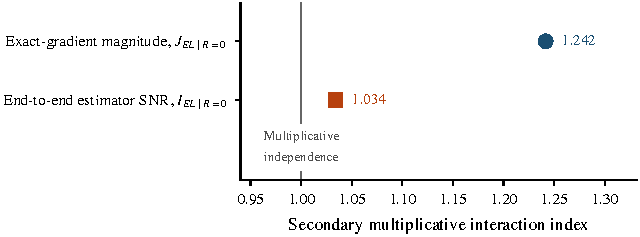
\includegraphics[width=0.64\textwidth]{figures/fig0_el_primary.pdf}
\caption{Primary $E\times L$ interaction evidence on the secondary
multiplicative scales. $J_{EL}=1.242$ corresponds to a 24.2\% super-additive
shift in RMS exact-gradient magnitude, whereas $I_{EL}=1.034$ corresponds to
a 3.4\% super-additive shift in RMS end-to-end estimator SNR. The vertical
reference at one denotes multiplicative independence. These descriptive
indices complement, rather than replace, the H1 and H2 mixed-model tests.}
\label{fig:el-primary}
\end{figure*}

\subsection{\texorpdfstring{H3---end-to-end estimator-SNR $E\times R$ interaction ($\beta_{ER}$)}{H3---end-to-end estimator-SNR E x R interaction}}

$\beta_{ER}=-0.000958$ (SE $0.007293$, $z=-0.13$), $p=0.896$, $p_{\mathrm{Holm}}=0.896$: \textbf{not rejected}. The estimate is close to zero, and the confirmatory analysis provides no evidence of an $E\times R$ interaction. This is not evidence of equivalence; no smallest effect of interest or equivalence test was prespecified. The final $n=443$ end-to-end bootstrap gives a percentile interval $[-0.030298,0.024478]$ (median $-0.001868$), consistent with the Wald/Holm non-rejection and the broader clean-null pattern for this coefficient; inclusion of zero is reported alongside, not in place of, the non-rejection decision. The $D\ge3$ sensitivity fit (block counts $3,4,6$ only, where $R$ can structurally matter---see Section~\ref{sec:residual-arch}) gives $-0.002128$ (SE $0.007004$, $p=0.761$), with extensive overlap between the confirmatory and sensitivity Wald confidence intervals.

\subsection{\texorpdfstring{H4---block-count-moderated $L\times R$ interaction ($\beta_{LRD}$)}{H4---block-count-moderated L x R interaction}}

$\beta_{LRD}=-0.010179$ (SE $0.005362$, $z=-1.90$), $p=0.0577$, $p_{\mathrm{Holm}}=0.115$: \textbf{not rejected}, but the closest of the three non-rejected hypotheses to the family-wise threshold. This is substantially different from how this coefficient looked before the mode-pooling fix (Appendix~\ref{app:verification}, A.5): under the (now-superseded) pooled fit, $\beta_{LRD}=+0.000511$, $p_{\mathrm{Holm}}=1.0$---a near-zero pooled estimate. The near-boundary character is specific to correctly restricting the fit to end-to-end-mode data.

Three further checks each pull against treating this near-boundary result as a likely real effect awaiting more data, without contradicting the Wald result outright (Figure~\ref{fig:h4-fragility} shows the depth- and mode-sensitivity checks side by side against the adopted confirmatory value):

\begin{itemize}
\item \textbf{Depth range}: the $D\ge3$ sensitivity fit shrinks the estimate to less than half its magnitude ($-0.00516$, SE $0.00673$, $p=0.443$)---the near-boundary character does not survive restricting to the block counts where $R$ is structurally active, indicating it depends on the low-block-count end of the full sweep.
\item \textbf{Mode sensitivity}: refitting per mode shows this is the coefficient with the most cross-mode tension in the entire model---conditional-only gives $+0.0104$ ($p=0.094$), end-to-end-only gives $-0.0102$ ($p=0.058$), opposite signs at comparable magnitude and precision. This is consistent with the pooled estimate's near-zero value reflecting partial cancellation between two effects moving in different directions under pooling, not a genuinely near-zero effect in either mode alone.
\item \textbf{Bootstrap}: the end-to-end-only run was extended to a final $n=443$ iterations (0 failed fits), well beyond the $n=40$ initial diagnostic. The final percentile interval, $[-0.026975,0.006403]$ (median $-0.010811$), still includes zero. This interval's shape stabilized earlier, across checkpoints, than the other two coefficients', but interval-shape stability is not the same as resolving the underlying near-boundary Wald result: the interval still straddles zero, so the extended bootstrap neither corroborates nor contradicts the Wald test's near-miss, consistent with every smaller $n$ reported for this coefficient. H4 remains genuinely inconclusive and fragile across depth range, estimator mode, and leave-one-initialization-out perturbation (Section~\ref{sec:results-robustness}) rather than a result awaiting simple confirmation from additional bootstrap iterations.
\end{itemize}

\begin{figure*}[t]
\centering
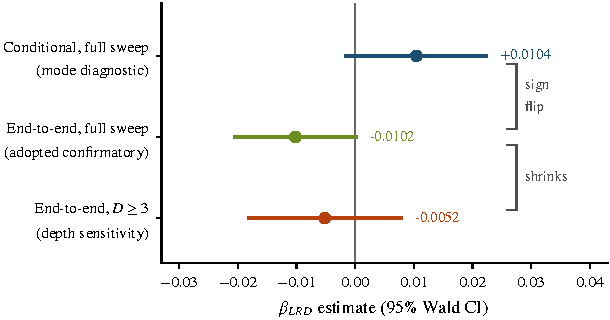
\includegraphics[width=0.72\textwidth]{figures/fig2_h4_fragility.pdf}
\caption{$\beta_{LRD}$ across three refits (95\% Wald CIs). The
conditional-only and end-to-end-only (adopted confirmatory) estimates sit
on opposite sides of zero at comparable magnitude and precision (top
bracket); restricting the adopted confirmatory fit to $D\ge3$ shrinks the
estimate to less than half its magnitude and moves it well away from the
significance boundary (bottom bracket). All three intervals include zero.}
\label{fig:h4-fragility}
\end{figure*}

Read together, H4 is not a hypothesis with a robust near-significant effect obscured by insufficient power; it is a hypothesis whose near-boundary character is itself fragile to the depth range analyzed and unresolved by resampling at the sample size achieved.

\subsection{Secondary and exploratory analyses}

None of the following are part of the Holm-corrected confirmatory family.

\textbf{Three-way interaction.} $\beta_{ELR}=-0.021315$ (SE $0.010287$, $p=0.0383$, end-to-end-only)---nearly double the now-superseded pooled magnitude ($-0.0111$), same sign, only narrow CI overlap. The unadjusted $p$-value crosses the nominal $0.05$ line; this changes nothing about the confirmatory family (the term was never submitted to Holm correction and is not being submitted now) and is reported for completeness rather than elevated into a new finding.

\textbf{Fold-change indices.} $I_{AB}$ (RMS-$\mathrm{SNR}_{\mathrm{est}}$-based, end-to-end-only primary) is super-additive for both $E\times L$ ($1.034$) and $E\times R$ ($1.010$), consistent in direction with the regression results above. $L\times R$ is a genuinely borderline case: $0.963$ (end-to-end-only), $0.997$ (pooled), $1.019$ (conditional-only)---all within $\sim$4\% of multiplicative independence, with the sub-/super-additive label flipping depending on which mode's data feeds it. This is reported as an unresolved borderline case, not a settled qualitative finding either way. The exact-gradient-based $J_{AB}$ is mode-invariant by construction ($1.242$, $1.184$, $0.992$ for $E{:}L$, $E{:}R$, $L{:}R$).

\textbf{Configuration-level SNR comparisons.} Configuration 3 (local cost alone) is the best single-intervention configuration in all 20 of 20 depth--budget cells tested, under both pooled and end-to-end-only data. Configuration 8 (all three interventions combined) exceeds it in only 4 of 20 cells under end-to-end-only data---down from 9 of 20 under the (superseded) pooled data, with the difference traced specifically to conditional-mode rows: the wins at block count 4 and at block count 6/budget 2000 disappear once conditional-mode rows are excluded, leaving only the block-count-3 cluster (unchanged across both; Figure~\ref{fig:q1-comparison} shows both grids side by side). Bundling all three interventions does not reliably outperform local cost alone. Final energy and global fidelity require no equivalent mode correction (verified by direct comparison: the relevant columns carry no \ttf{analysis\_mode} dependence and are numerically identical between the old and new tables)---but these values describe untrained initial states only, since the confirmatory design measures at matched initial parameters before any optimizer step; no claim about training or convergence quality follows from them.

\begin{figure*}[t]
\centering
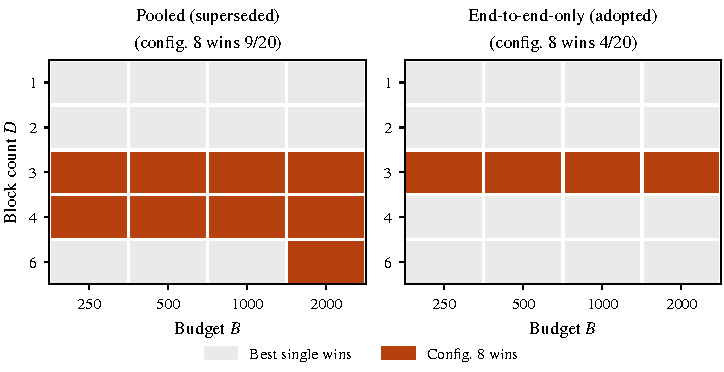
\includegraphics[width=0.7\textwidth]{figures/fig5_q1_comparison.pdf}
\caption{Depth--budget grid showing where configuration 8 (all three
interventions) exceeds the best single-intervention configuration on RMS
$\snrest$, under pooled (superseded) data (left) and the adopted
end-to-end-only data (right). The win count narrows from 9/20 to 4/20, and
the surviving wins collapse to the block-count-3 cluster once
conditional-mode rows are excluded.}
\label{fig:q1-comparison}
\end{figure*}

\subsection{Estimator fidelity, entanglement, energy, fidelity, and resource cost}

\textbf{Entanglement.} $E=1$ produces substantially lower entropy ($\sim0.32$--$0.42$) and higher purity ($\sim0.83$--$0.87$) than $E=0$ ($\sim0.75$--$0.82$ entropy, $\sim0.64$--$0.67$ purity) at every tested block count---validating the restricted-entanglement label (Figure~\ref{fig:entanglement-diagnostic}). Reported error bars are real per-initialization standard errors ($n=50$ per $(E,R,D)$ cell; see Appendix~\ref{app:verification}, A.3, for the correction that produced them). A mixed-model regression of entropy on centered block count, fit separately per $E$ value, finds no trend distinguishable from zero for either ($p\approx0.30$--$0.35$, cross-checked against cluster-robust OLS by initialization)---``flat, not trending'' holds on solid footing, consistent with the self-contained per-block architecture (Section~\ref{sec:residual-arch}): no mechanism exists for entanglement to accumulate across blocks. $R$'s effect on this diagnostic is exactly zero at block counts $1,2$ and appears only from block count $3$ onward, matching the residual-activation boundary condition exactly rather than approximately.

\begin{figure*}[t]
\centering
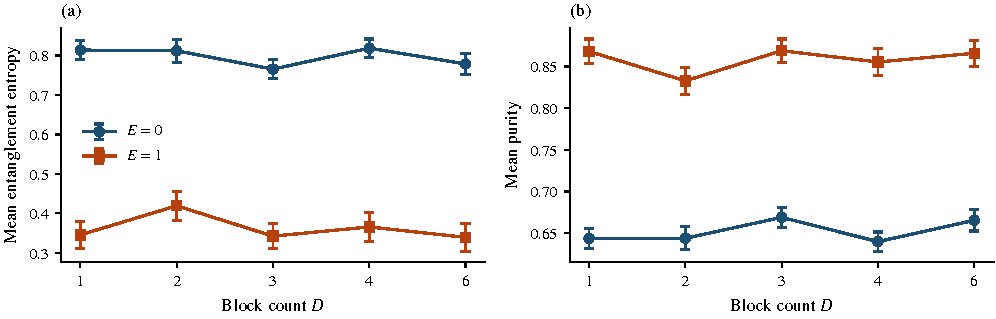
\includegraphics[width=0.92\textwidth]{figures/fig3_entanglement.pdf}
\caption{Mean entanglement entropy (a) and purity (b) by block count $D$,
for $E=0$ and $E=1$, marginalized over $R$ (whose effect on this diagnostic
is exactly zero at $D\in\{1,2\}$ and small even from $D=3$ onward). Error
bars are per-initialization SEMs ($n=50$). Both series are flat
across $D$ within uncertainty, consistent with the self-contained
per-block architecture.}
\label{fig:entanglement-diagnostic}
\end{figure*}

\textbf{Bias and sign agreement.} Split by mode, conditional mode has higher sign agreement and lower absolute bias than end-to-end mode in all 8 of 8 configurations, with no exceptions (Figure~\ref{fig:mode-split-bias}): pooled sign agreement is $0.842$, but conditional-only is $0.869$ against end-to-end-only's $0.814$; pooled median absolute bias is $0.00329$, against conditional-only's $0.00265$ and end-to-end-only's $0.00416$. The gap widens at higher-bias configurations. This pattern is consistent across all eight configurations and is compatible with the expected effect of additional forward-feature re-estimation in end-to-end mode. It also offers a plausible, but not independently causal, explanation for why the depth- and three-way terms ($\beta_{LRD}$, $\beta_{ELR}$) show greater cross-mode sensitivity than the simpler two-way terms.

\begin{figure*}[t]
\centering
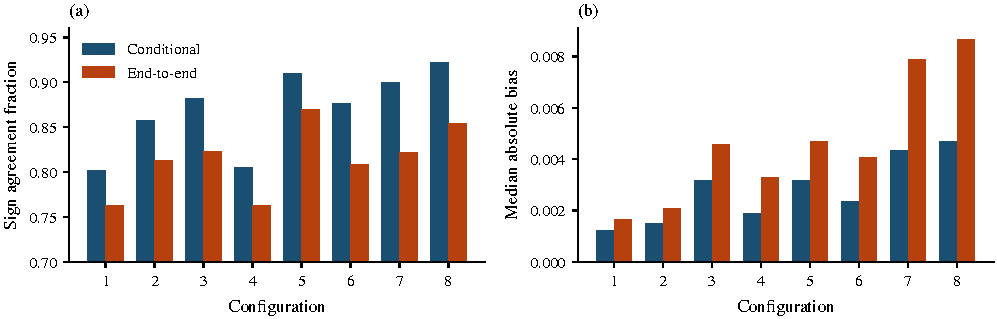
\includegraphics[width=0.92\textwidth]{figures/fig4_mode_split_bias.pdf}
\caption{Sign agreement (a) and median absolute bias (b) by configuration,
conditional vs. end-to-end mode. Conditional mode beats end-to-end mode on
both properties in all 8 of 8 configurations, with no exceptions; the bias
gap widens at higher-bias configurations (7, 8).}
\label{fig:mode-split-bias}
\end{figure*}

\textbf{Resource accounting.} The shot-budget parameter $B$ is a single total budget, floor-divided (with a deterministic one-shot-at-a-time remainder) across every measurement job required for one replicate's complete gradient vector. Total shots are therefore always exactly matched at fixed nominal $B$ (zero unused remainder in every cell), but realized shots per circuit are not: the local-cost objective's two observable bases (versus the global objective's one) and end-to-end mode's additional forward-feature jobs both increase the job count at fixed $B$, so local-cost and end-to-end-mode configurations receive systematically fewer shots per circuit than global-cost/conditional-mode configurations at the same nominal budget and block count---a gap that widens with block count (a $\sim$27\% difference in circuit count between the two extremes at block count 6). ``Matched total measurement budgets'' therefore holds exactly for total shot count, but not for per-circuit measurement precision; this paper avoids the unqualified claim accordingly.

\subsection{Robustness and implementation checks}
\label{sec:results-robustness}

Table~\ref{tab:confirmatory-summary} summarizes the four confirmatory hypotheses, and Figure~\ref{fig:confirmatory-forest} compares their Wald intervals with the achieved bootstrap diagnostics. Appendix~\ref{app:verification} documents gradient validation (A.1), block semantics (A.2), the entanglement-diagnostic correction (A.3), the residual activation boundary (A.4), and the discovery and correction of inadvertent mode pooling in the confirmatory fitting path (A.5). Every other check summarized below---optimizer refits, residual diagnostics, leave-one-initialization-out influence, the $D=1$/zero-variance checks of Section~\ref{sec:zero-variance-sensitivity}, and the bootstrap extension---is traceable to its verification script and record file through the reproducibility index (Table~\ref{tab:repro-index}) rather than restated in prose here. The mode-pooling correction materially changed H4's estimate and interpretation while leaving the family-level rejection pattern unchanged.

\textbf{Model convergence and optimizer agreement.} The adopted end-to-end full-sweep H2--H4 fit converges (\ttf{singular\_fit=False}; neither the group-intercept nor the nested-parameter variance component is within $10^{-8}$ of zero) and emits one pre-existing convergence warning (the MLE sits near, not strictly on, a parameter-space boundary), unchanged from every other fit in this study that uses the same formula. Refitting with an independent optimizer (BFGS in place of the default L-BFGS, identical formula, data, coding, and likelihood) reproduces $\beta_{EL}$, $\beta_{ER}$, and $\beta_{LRd}$ to 8--9 significant figures and the log-likelihood and random-effect variances to approximately five significant figures---no meaningful optimizer sensitivity.

\textbf{Residual diagnostics.} The adopted fit shows systematic, not merely incidental, heteroscedasticity: residual standard deviation falls from approximately $0.659$ at $D=1$ to $0.276$ at $D=6$, and rises from approximately $0.301$ at $B=250$ to $0.513$ at $B=2000$---opposite directions, both monotonic. Standardized residuals are moderately heavy-tailed (approximately $1.14\%$ exceed absolute value 3, roughly four times the normal-theory expectation). These diagnostics are a real caveat on model-based Wald standard errors, which assume homogeneous residual variance: the reported SEs may be mildly optimistic in low-block-count or high-budget regions specifically. They are not grounds for discarding the fit, which converges cleanly, is non-singular, and is optimizer-independent as above; no heteroscedasticity-robust mixed-model refinement was added post hoc.

\textbf{Leave-one-initialization-out influence.} Refitting the adopted model 50 times, each time excluding one complete initialization (all 50 converged, zero failures), finds no sign reversal for $\beta_{EL}$ or $\beta_{LRd}$ under any single deletion, and $\beta_{EL}$ remains $p<0.05$ (raw) in all 50 deletions---H2's rejection is not attributable to any one initialization. The largest single deletion (initialization 1) shifts $\beta_{EL}$ by $1.131$ original-standard-error units; this magnitude shift is flagged, not dismissed---$\beta_{EL}$'s sign and rejection direction are stable across every deletion, while its point estimate is more sensitive to individual initializations than the other two coefficients. $\beta_{ER}$ shows 16 of 50 sign flips but is never near significance in either direction, consistent with a coefficient centered near zero. $\beta_{LRd}$ shows 18 of 50 (36\%) raw-$p$ crossings of $0.05$ relative to its already-borderline full-data value---the most fragile of the three coefficients by this diagnostic, and a fourth independent line of evidence (alongside depth range, estimator mode, and the extended bootstrap) that H4's near-boundary character is not a robust feature of the data. Figure~\ref{fig:residual-diagnostics} shows the residual and convergence diagnostics; Figure~\ref{fig:initialization-influence} shows all 50 leave-one-initialization-out estimates against the full-data reference for all three coefficients.

\begin{figure}[t]
\centering
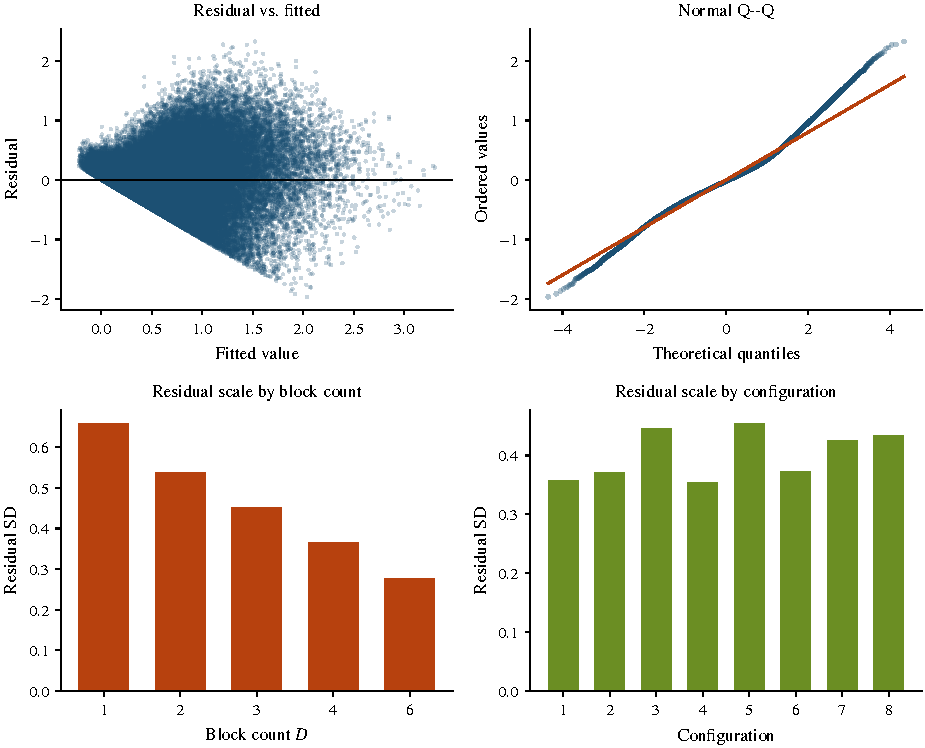
\includegraphics[width=\columnwidth]{figures/fig8_model_residual_diagnostics.pdf}
\caption{Adopted H2--H4 fit diagnostics: residual-versus-fitted (a), normal
Q--Q (b), residual standard deviation by block count (c), and by
configuration (d). Residual spread falls with block count and rises with
shot budget (not shown in the same panel scale; reported in text), and the
Q--Q plot shows mild positive-tail heaviness relative to a normal
reference. These are reported as caveats on Wald standard errors, not as
evidence against the fit, which converges, is non-singular, and is
optimizer-independent (main text).}
\label{fig:residual-diagnostics}
\end{figure}

\begin{figure}[t]
\centering
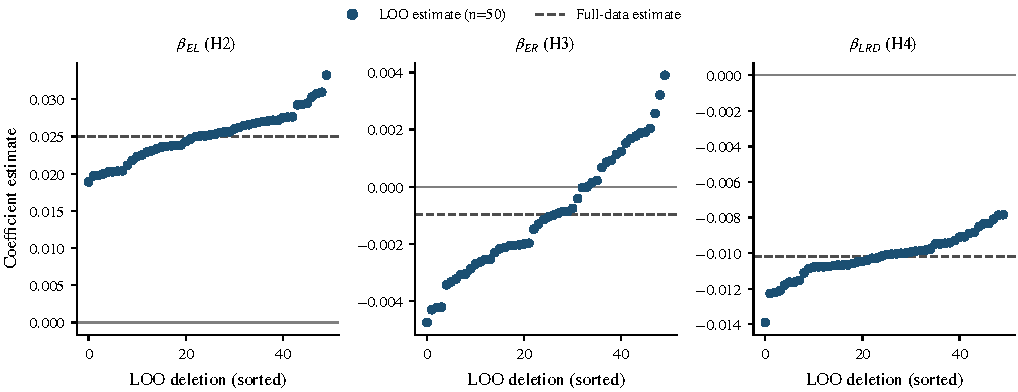
\includegraphics[width=\columnwidth]{figures/fig9_initialization_influence.pdf}
\caption{Leave-one-initialization-out estimates (sorted, $n=50$ deletions)
for $\beta_{EL}$, $\beta_{ER}$, and $\beta_{LRd}$, against the full-data
reference (dashed). $\beta_{EL}$ never crosses zero and remains
raw-$p<0.05$ in every deletion; $\beta_{ER}$ straddles zero symmetrically,
consistent with a clean null; $\beta_{LRd}$ remains entirely negative but
shows the widest relative spread of the three, consistent with its
near-boundary fragility.}
\label{fig:initialization-influence}
\end{figure}

\begin{table*}[t]
\centering
\footnotesize
\setlength{\tabcolsep}{3pt}
\renewcommand{\arraystretch}{1.12}
\begin{tabularx}{\textwidth}{@{}llrrrr>{\raggedright\arraybackslash}Xcc@{}}
\toprule
Hyp. & Coef. & Est. & SE & $p$ & $p_{\mathrm{Holm}}$ & Bootstrap 95\% interval ($n$) & \shortstack{Wald/Holm\\decision} & \shortstack{Bootstrap\\support} \\
\midrule
H1 & $\eta_{EL}$ & $0.00435$ & $0.00153$ & $0.0045$ & $0.0134$ & $[0.00081,0.00803]$ (400) & Reject & Yes \\
H2 & $\beta_{EL}$ & $0.02500$ & $0.00728$ & $0.0006$ & $0.0024$ & $[-0.01802,0.06569]$ (443) & Reject & No \\
H3 & $\beta_{ER}$ & $-0.00096$ & $0.00729$ & $0.896$ & $0.896$ & $[-0.03030,0.02448]$ (443) & Not rejected & N/A$^\dagger$ \\
H4 & $\beta_{LRD}$ & $-0.01018$ & $0.00536$ & $0.0577$ & $0.115$ & $[-0.02698,0.00640]$ (443) & Not rejected & N/A$^\dagger$ \\
\bottomrule
\end{tabularx}
\caption{Confirmatory summary for the adopted end-to-end analysis. The formal decision column follows the prespecified Wald tests with Holm correction; the bootstrap column is diagnostic and does not replace it. H1's $n=400$ bootstrap independently corroborates its rejection. The $n=443$ H2--H4 bootstrap (extended from an initial $n=40$ diagnostic, with 0 failed fits and more than the required minimum of 400 iterations) does not corroborate H2's rejection; this pattern remained stable as the bootstrap was extended rather than narrowing with more iterations. $^\dagger$H3 and H4 have no confirmatory rejection to corroborate. Their intervals include zero, which is consistent with, but does not prove, non-rejection because equivalence was not tested.}
\label{tab:confirmatory-summary}
\end{table*}

\begin{figure}[t]
\centering
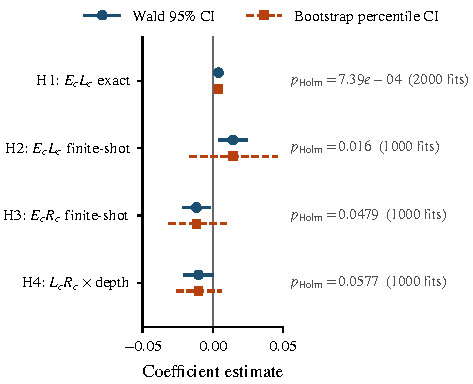
\includegraphics[width=\columnwidth]{figures/fig1_confirmatory_forest.pdf}
\caption{Prespecified Wald 95\% confidence intervals (solid, circles)
and achieved bootstrap percentile diagnostics (dashed, squares), with
Holm-adjusted $p$-values. H1 used $n=400$ bootstrap iterations. The adopted
end-to-end H2--H4 reruns reached a final $n=443$ (extended from an initial
$n=40$ diagnostic). H2's Wald interval excludes zero while its percentile
bootstrap interval includes zero; this difference is reported rather than
resolved by selecting one method, and the prespecified Wald/Holm decision
remains the confirmatory one. Figure~\ref{fig:bootstrap-stability} shows
how these intervals evolved across the extension.}
\label{fig:confirmatory-forest}
\end{figure}

\begin{figure}[t]
\centering
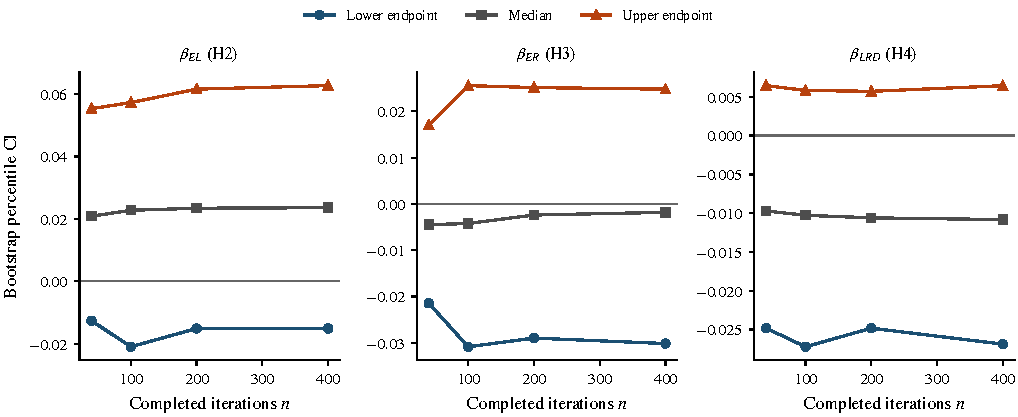
\includegraphics[width=\columnwidth]{figures/fig10_bootstrap_endpoint_stability.pdf}
\caption{Lower endpoint, median, and upper endpoint of the H2--H4
percentile bootstrap intervals at each completed-iteration checkpoint
($n=40,100,200,400,443$), from the same extension summarized in
Table~\ref{tab:confirmatory-summary}. $\beta_{EL}$'s interval continued to
include zero throughout and did not narrow or move away from zero as
iterations increased; $\beta_{LRd}$'s interval also continued to straddle
zero. Each checkpoint is a snapshot of the same accumulating resampling
distribution, not an independent hypothesis test, and no convergence claim
beyond what these machine-readable checkpoints show is inferred from visual
inspection alone.}
\label{fig:bootstrap-stability}
\end{figure}

\section{Discussion}

\subsection{Summary and effect-size interpretation}

Two of the four confirmatory hypotheses are rejected under the prespecified Wald/Holm procedure and two are not. H1 and H2 have the same positive direction, providing model-based evidence of a super-additive $E\times L$ interaction in both exact-gradient magnitude and end-to-end estimator SNR. The achieved $n=443$ end-to-end bootstrap did not independently corroborate H2, stably rather than as an artifact of too few iterations, so the finite-shot result should be read as Wald/Holm-supported and sign-stable across sensitivity analyses rather than as confirmed by two inferential procedures. On the secondary multiplicative indices, the interaction corresponds to a 24.2\% shift in RMS exact-gradient magnitude ($J_{EL}=1.242$) and a 3.4\% shift in RMS $\snrest$ ($I_{EL}=1.034$): directionally consistent, but operationally modest on the SNR scale (Figure~\ref{fig:el-primary}). H3 yields an estimate close to zero and no evidence of an $E\times R$ interaction, although equivalence was not tested. H4 is not rejected, and its proximity to the unadjusted threshold is fragile to the analyzed depth range, estimator mode, and leave-one-initialization-out perturbation; the $n=443$ bootstrap remains genuinely inconclusive rather than a result awaiting more resampling.

\subsection{Evaluation of the mechanistic prior}

The companion review's directional expectation was that restricted entanglement and the local TFIM-energy objective would interact \emph{sub-additively} at the exact-gradient level: an architecture that already preserves locally relevant derivative structure might leave the local objective less marginal signal to add \cite{shen2026gradient}. The data contradict that expectation. $\eta_{EL}$ is positive, and the same direction appears in the estimator-SNR analysis. The result is therefore not evidence that the two interventions merely duplicate a shared mechanism. Within this architecture, restricting within-block correlation spreading and changing which reduced-state derivatives enter the objective appear to reinforce one another.

That interpretation should remain local to the implemented model. Theoretical connections among expressibility, entanglement, and observable support do not imply a universal sign for an empirical interaction coefficient \cite{holmes2022expressibility,ortizmarrero2021entanglement,ragone2024lie}. The present $E$ factor changes a specific four-CNOT schedule, and the $L$ factor changes the full objective from global infidelity to normalized TFIM energy. The positive interaction therefore motivates a mechanistic hypothesis for follow-up work rather than establishing a general theorem about restricted entanglement and local costs.

No directional prior was assigned to interactions involving the residual shortcut. H3's near-zero estimate and H4's fragile, depth- and mode-sensitive estimate are consequently open empirical results rather than failed confirmations of a residual-network theory.

\subsection{Relation to prior trainability and finite-shot literature}

The exact-gradient result extends two previously separate observations. Local objectives can improve gradient scaling under specified circuit-depth assumptions \cite{cerezo2021costfunction}, and excessive random entanglement can suppress gradients \cite{ortizmarrero2021entanglement,patti2021entanglement}. The super-additive $E\times L$ coefficient shows that, in this finite four-qubit architecture, the benefit associated with the objective does not diminish after entanglement is restricted. This interaction-aware result is compatible with broader theoretical work that treats architecture, state structure, and observable support as coupled determinants of loss concentration \cite{ragone2024lie}, while remaining far too small in scale to test that theory's asymptotic claims.

The results also reinforce the distinction between gradient resolvability and full trainability. A nonvanishing or statistically resolvable initial gradient is neither necessary nor sufficient for successful convergence; shallow models can remain difficult because of traps, data-dependent concentration, or optimization dynamics \cite{anschuetz2022traps,thanasilp2023subtleties}. Conversely, mitigation methods based on identity initialization or layerwise growth act over an optimization trajectory rather than only at matched initial parameters \cite{grant2019identity,skolik2021layerwise}. The present findings should therefore be read as evidence about the quality of an initial finite-shot update signal, not as a ranking of end-to-end training algorithms.

ResQNets reported improved training behavior from residual shortcuts over full optimization trajectories \cite{kashif2024resqnets}. This study asks a narrower question: whether a fixed-gain shortcut between independently reset quantum blocks changes gradient resolvability at matched initial parameters. The absence of a detected $E\times R$ interaction and the fragility of the $L\times R\times D$ term do not contradict the ResQNet results. The architectures, estimands, and stages of training differ, and work on dissipative and pooling-based QNNs similarly shows that trainability guarantees do not transfer automatically across hybrid causal structures \cite{beer2020training,sharma2022dissipative,pesah2021qcnn}.

The finite-shot findings connect directly to measurement-aware optimization. Adaptive-shot methods allocate samples according to estimated gradient means and variances \cite{kubler2020adaptive,tamiya2022stochastic}, while variance-reduction and gradient-acquisition studies show that the number and organization of measurements can materially alter optimization cost \cite{kreplin2024finite,chinzei2025tradeoff,bowles2025backpropagation}. Here, a fixed total budget does not imply equal shots per circuit, because objective decomposition and forward-feature re-estimation change the number of measurement jobs. The observed bias and sign-agreement gap between conditional and end-to-end modes further shows that node-level derivative precision does not by itself characterize the estimator supplied to an optimizer.

Finally, the zero-variance exclusion pattern exposes a limitation specific to plug-in SNR estimation. All excluded cells occur under the global-cost condition, making the finite-shot $E\times L$ model conditional on factor-dependent eligibility. The sign stability of $\beta_{EL}$ under reported sensitivity checks is reassuring but does not identify the mechanism or eliminate selection concerns. This caveat is one reason the exact-gradient interaction, which does not depend on that exclusion process and is corroborated by the matched bootstrap, remains the paper's strongest result.

\subsection{Implications for interaction-aware QML evaluation}

The results illustrate why QNN interventions should not be evaluated only by removing or adding one component at a time. The local TFIM-energy objective is the best single intervention in every tested depth--budget cell, yet the positive $E\times L$ interaction shows that the effect of restricted entanglement depends on which objective is used. Conversely, the fully combined configuration does not reliably outperform the best single intervention. Pairwise reinforcement therefore does not imply that adding all available strategies produces the best system.

The finite-shot analyses also show that the definition and implementation of an evaluation metric are part of the computational experiment. Matching total shots does not match shots per circuit; re-estimating intermediate features changes estimator bias and sign reliability; and a plug-in SNR estimator can create factor-dependent eligibility when replicate variance is estimated as exactly zero. The post-run mode-pooling correction further demonstrates that prespecified statistical models do not by themselves guarantee a valid computational analysis. Explicit data-mode guards, deterministic seed management, frozen inputs, independent gradient checks, and regression tests are therefore treated here as components of the evaluation protocol rather than as ancillary software details.

\subsection{Scope, limitations, and analysis provenance}

All findings are scoped to a single four-qubit implementation within the companion review's proposed 2--10-qubit regime \cite{shen2026gradient}. The study evaluates one open-boundary TFIM task at $J=1$ and $h=0.5$, a noiseless statevector simulator with no hardware-noise model, and one implementation each of restricted entanglement, local cost, and residual connections. No claim generalizes to other qubit counts, other ansätze, other tasks, or different implementations of the same three interventions, and no claim is made about asymptotic barren-plateau scaling class, which this design was never positioned to test. The cost-function contrast is the full difference between normalized TFIM energy and global target-state infidelity, not measurement locality in isolation. The self-contained, measure--re-encode--reset block architecture (Section~\ref{sec:ansatz}) is a specific hybrid design choice, not representative of arbitrary layered variational circuits with a single continuously evolving state. The $D\ge3$ sensitivity analysis for H3/H4 is a post-run addition that does not redefine the confirmatory population, even where it materially changes the interpretation of a near-boundary result (H4). Block-count-1 estimates carry wider uncertainty than deeper block counts, since the replicate-count calibration criterion did not converge there even at a substantially raised ceiling.

The planned $D=1$-exclusion and exclusion-rate sensitivity checks (Section~\ref{sec:zero-variance-sensitivity}) have since been completed, and the zero-variance selection concern they were meant to address turned out to be more serious than initially anticipated: exclusion is not merely concentrated at $D=1$, it is exactly confined to $L=0$ across the entire design, in both estimator modes. $L$ is one of the two factors in the paper's headline $E\times L$ interaction, so the confirmatory estimator-SNR model is conditional on an eligibility process perfectly associated with cost type. This does not establish that $\beta_{EL}$ is biased by it---the $D=1$-exclusion refit moves $\beta_{EL}$ \emph{away} from, not toward, zero, the opposite of what a spurious, exclusion-driven signal would be expected to do---but the completed analysis does not rule out a subtler mechanism either, and the selection process's physical or computational origin remains uninvestigated. $\beta_{EL}$ also shifts by approximately $1.0$--$1.1$ original standard errors under two independent perturbations (excluding $D=1$; deleting the single most influential initialization), a magnitude worth carrying forward as an open precision/influence caveat even though neither perturbation reverses its sign or its rejection status. The adopted end-to-end H2--H4 bootstrap was extended to a final $n=443$ (Section~\ref{sec:results-robustness}), exceeding the required minimum of 400 but short of the preferred target of 1000; at this achieved scale, the bootstrap does not independently corroborate H2 and remains inconclusive for H4, a pattern that held stably across the extension rather than resolving with more iterations. Residual diagnostics on the adopted fit also show real heteroscedasticity by block count and budget and moderately heavy tails (Section~\ref{sec:results-robustness}), meaning the model-based Wald standard errors rest on an imperfect homogeneous-residual approximation; no heteroscedasticity-robust or other variance-modeling refinement was undertaken. Finally, every result here is from noiseless simulation; no hardware-noise experiment was performed.

An important procedural limitation emerged during the post-run audit: the originally reported confirmatory H2--H4 numbers had silently pooled two estimator modes that the Methods section designates as confirmatory and diagnostic-only, because the fitting code carried no mode-awareness. This was not caught by any built-in check---only by an independent verification pass performed after the confirmatory run. Correcting it left the overall reject/non-reject pattern unchanged but materially altered H4's character (Section~\ref{sec:results-robustness}) and every H2--H4 bootstrap result. This episode is reported in full (Appendix~\ref{app:verification}, item A.5) rather than folded quietly into a revised number, and is itself evidence for a broader point: an operational, finite-sample framework of the kind this paper and the companion review propose \cite{shen2026gradient} is only as trustworthy as the implementation-level checks built around it, and those checks are worth building deliberately rather than relying on a post hoc audit to catch what a prespecified analysis plan does not.

\subsection{Implications for the SNR framework and future work}

Independent of which specific hypotheses were rejected, this paper demonstrates that the companion review's SNR-based reframing is executable in a four-qubit instance within its proposed few-qubit regime, and that doing so surfaces genuine, sometimes surprising empirical content---most notably a super-additive $E\times L$ interaction running counter to the review's own interpretive prior \cite{shen2026gradient}, and a residual-connection interaction (H4) whose apparent near-significance turns out not to be a robust feature of the data once probed from several directions. The audit episode instead shows that measurable outcomes and a prespecified analysis plan are not sufficient by themselves: substantively different estimator modes require explicit filtering, assertions, and regression tests at the implementation level. The corrected mode split also became scientifically informative by revealing that the simpler $E\times L$ term is comparatively stable across modes whereas depth-related terms are more sensitive.

Several directions follow directly from this study's scope limits. A continuous-state (non-self-contained-block) control experiment for the $E\times L$ comparison would clarify whether the super-additive interaction found here is a property of the measure--re-encode--reset architecture specifically or would carry over to conventional layered circuits with a single evolving state. A hardware-noise study is a natural next step, since every result here is from noiseless simulation. Testing additional residual-connection implementations (variable or trainable gain, alternative shortcut placements) and additional local-objective formulations would clarify whether H3's near-zero estimate and H4's fragile signal are properties of this specific fixed-gain design or would look different under other reasonable choices. Finally, extending to larger qubit counts with adequate theoretical support---rather than a numerical sweep alone---remains the only way to connect this few-qubit operational picture back to the asymptotic barren-plateau question that motivated it in the first place.

\section{Conclusion}\label{sec:conclusion}

This study uses a complete $2^3$ factorial protocol to evaluate three QNN gradient-resolvability strategies under matched finite-shot budgets. The protocol separates exact-gradient signal, estimator resolvability, bias, sign reliability, task metrics, and measurement cost while preserving the matched structure needed to estimate whether interventions reinforce, duplicate, or interfere with one another.

In the four-qubit measure--re-encode--reset case study, restricted entanglement and the TFIM-energy objective exhibit a positive exact-gradient interaction supported by both mixed-effects and matched-bootstrap analyses. The analogous finite-shot estimator-SNR interaction has the same direction but is modest in multiplicative magnitude, is not corroborated by the achieved bootstrap, and is conditional on a factor-dependent zero-variance exclusion process. No robust interaction involving the fixed residual shortcut is identified, and combining all three strategies does not consistently outperform the best single intervention.

The main conclusion is methodological as well as empirical: QNN trainability interventions should be treated as potentially interacting components rather than assumed to compose additively. At the same time, exact-gradient magnitude, finite-shot resolvability, estimator fidelity, and optimization performance are distinct outcomes and should not be collapsed into a single claim of ``trainability.'' The released code, frozen data, audit records, and regression tests provide a reproducible basis for extending the protocol to continuous-state architectures, hardware-noise models, optimization trajectories, alternative objectives and residual designs, and larger qubit counts.

\backmatter

\section*{Statements and Declarations}

\bmhead{Funding} No external funding was received.

\bmhead{Competing interests} The author declares no financial or non-financial competing interests.

\bmhead{Ethics approval} Not applicable. This study used computational simulations and did not involve human participants, human data, animals, or biological materials.

\bmhead{Consent to participate} Not applicable.

\bmhead{Consent for publication} Not applicable.

\bmhead{Author contributions} Brandon Shen conceived the study, implemented the simulation and analysis pipeline, conducted the experiments and verification analyses, interpreted the results, prepared the figures, and wrote and revised the manuscript.

\bmhead{Data availability} The public repository contains the exact production data behind every reported number and figure, organized under \ttf{results/} into five clearly separated, explicitly labeled directories: \ttf{production\_confirmatory/} (the adopted end-to-end-mode raw per-replicate simulation tables in \ttf{raw/\{exact,finite\_shot\_end\_to\_end,finite\_shot\_conditional\}.parquet}, the aggregated pointwise gradient/SNR statistics in \ttf{pointwise\_gradient\_statistics.parquet}, the confirmatory coefficient and hypothesis tables, the exact production config, and all report figures), \ttf{production\_corrected\_end\_to\_end/} (the end-to-end-only nested-bootstrap arm, $n=443$), \ttf{superseded\_pooled/} (the pre-fix pooled-mode coefficient tables, kept for reference and never presented as current -- see Appendix~\ref{app:verification}, A.5), \ttf{sensitivity\_analyses/} (D=1-exclusion, leave-one-initialization-out, zero-variance-audit, and optimizer-comparison outputs), and \ttf{smoke\_test/} (non-reportable pipeline-exercise runs, explicitly marked not for scientific use). Each production directory includes a \ttf{SHA256SUMS.txt} of its frozen files. The commit at which this manuscript's numbers were finalized is recorded in \ttf{MANUSCRIPT\_COMMIT.txt} at the repository root. The repository is available at \url{https://github.com/Brandon-Shen/few-qubit-qnn-snr}.

\bmhead{Code availability} The public repository contains the quantum-simulation and gradient-assembly code, mixed-model and multiplicity-correction code, production and memory-efficient nested-bootstrap implementations, figure-generation scripts, and the regression-test suite. The code is available at \url{https://github.com/Brandon-Shen/few-qubit-qnn-snr}.

\bmhead{Materials availability} Not applicable.

\bmhead{Software availability and reproducibility information} Analyses were run with Python 3.12.10, pandas 3.0.3, numpy 2.5.1, statsmodels 0.14.6, scipy 1.18.0, and matplotlib 3.11.0. Mixed-effects models use REML and an L-BFGS-first optimizer fallback (Methods); an independent BFGS refit of the adopted H2--H4 model reproduced every target coefficient to 8--9 significant figures (Section~\ref{sec:results-robustness}). A fit is flagged singular if either variance component is within $10^{-8}$ of zero; every confirmatory and sensitivity fit in this paper converged and none was singular, though several (including the adopted fit) emitted a non-blocking convergence warning indicating the MLE sits near a parameter-space boundary, a documented pre-existing property of this model/data combination. Random seeds throughout the pipeline are derived deterministically from a root seed, a named stream, and integer/string ids via SHA-256 (\ttf{qnn\_snr.seeds.derive\_seed}), so any specific cell's numbers can be reproduced independently given the same root seed and config. Item-level provenance for every verification script, its inputs, and its outputs is given in the reproducibility index (Table~\ref{tab:repro-index}) and the archived \ttf{verification/*.md} records in the code repository.

\appendix

\section{Implementation and Inference Audit Log}
\label{app:verification}

This appendix reports the checks that materially inform how the confirmatory results in Section~\ref{sec:results-robustness} should be interpreted. Purely computational or infrastructural detail (bootstrap sharding, memory management, concurrency, and script-level provenance) that does not change a scientific conclusion is not narrated here; it is indexed in Table~\ref{tab:repro-index} and archived in full in the code repository's \ttf{verification/*.md} records, consistent with the Data and Code availability statements. Checks added after inspection of the confirmatory outputs are labeled post-run and are not used to redefine the original hypothesis family (Section~\ref{sec:provenance}).

\medskip \noindent\textbf{A.1---Finite-difference validation of the H1 gradient chain rule.} Black-box central finite differences were computed on the full multi-block hybrid cost at 224 parameter-level comparisons: 16 matched points, block counts $D\in\{1,6\}$, and configurations 1, 2, 3, and 5. The worst relative error was $1.27\times10^{-5}$ overall and $9.77\times10^{-7}$ among non-floor-dominated rows, with the expected $O(h^2)$ truncation regime before floating-point saturation. An apparent sign reversal in an initial 16-point subsample was traced to small-sample noise: an ad hoc $E{:}L{:}\widetilde D$ term fit on the full 25{,}600-row exact dataset was small and not distinguishable from zero (post-run diagnostic, not a confirmatory test).

\medskip \noindent\textbf{A.2---Block-semantics resolution.} The implementation uses self-contained quantum blocks connected only by classical features, consistent with the node notation $z^{(\ell)}=q_\ell(x^{(\ell)},\theta^{(\ell)})$ and the total-gradient formula used in the analysis; a continued-state alternative tested during development did not agree with black-box finite differences. The companion review contains prose suggesting register-wide propagation across multiple layers \cite{shen2026gradient}; that language is not fully compatible with a reset-per-block architecture and is treated as an underspecification of the source framework, not evidence that entanglement persists between blocks in this experiment.

\medskip \noindent\textbf{A.3---Entanglement diagnostic correction.} A first-pass entropy/purity summary used across-condition spread (across the four configurations sharing a given $E$) rather than across-initialization standard errors, understating point-estimate uncertainty by roughly an order of magnitude, and is not used for inference. The corrected per-initialization analysis ($n=50$ real initializations per $(E,R,D)$ cell) is the one reported in Section~\ref{sec:results-robustness}'s companion diagnostic (``Entanglement'' paragraph, Figure~\ref{fig:entanglement-diagnostic}) and found real per-initialization standard deviations of $\sim0.15$--$0.27$ entropy units. The large, block-count-independent separation between $E=0$ and $E=1$ entropy/purity is unaffected by this correction and remains the primary validation that the restricted-entanglement label reflects a real difference in prepared states.

\medskip \noindent\textbf{A.4---Residual activation boundary.} The boundary convention $z^{(0)}=0$ implies the shortcut is inactive for $D\in\{1,2\}$ and first enters $x^{(3)}$ when $D=3$ (Section~\ref{sec:residual-arch}). A direct comparison of matched outputs confirmed numerical identity between $R=0$ and $R=1$ at the two structurally inactive block counts and divergence from $D=3$ onward, motivating the labeled $D\ge3$ sensitivity analyses reported for H3/H4 without replacing the prespecified full-sweep models.

\medskip \noindent\textbf{A.5---Mode-pooling bug: discovery, fix, and downstream consequences.} A post-run audit found that the H2--H4 confirmatory fit had been silently pooling \ttf{finite\_shot\_conditional} and \ttf{finite\_shot\_end\_to\_end} rows into one model, because the fitting code carried no \ttf{analysis\_mode} awareness and nothing upstream filtered to a single mode before fitting. This contradicted the Methods section's own stated design (end-to-end confirmatory, conditional diagnostic-only) and affected every H2--H4 coefficient and bootstrap iteration computed before the fix. The correction added an explicit guard---any fit call on multi-mode data now raises an error unless a caller-supplied \ttf{pool\_modes=True} opt-in is given---and updated every production call site to filter to end-to-end mode by default, with conditional-mode analysis moved to a separate, explicitly diagnostic code path that never writes to the confirmatory output files. A dedicated regression test reproduces the original bug against the pre-fix code and passes against the fixed code; the guarded fitting path was then rerun for real (not copied from prior derivation) and reproduced the independently derived end-to-end-only estimates to machine precision. The pooled-data files are retained, clearly marked as superseded, rather than deleted, because the mode-sensitivity pattern is itself a reportable finding: refitting separately by mode shows $\beta_{EL}$ is robust across modes (same sign, overlapping magnitude, both individually significant), whereas $\beta_{LRD}$ and the exploratory three-way term are not---conditional-only $\beta_{LRD}=+0.0104$ ($p=0.094$) versus end-to-end-only $\beta_{LRD}=-0.0102$ ($p=0.058$), opposite signs at comparable magnitude and precision (Section~\ref{sec:results-robustness}, Figure~\ref{fig:h4-fragility}). The reject/non-reject pattern across H1--H4 is unchanged by the correction, but H4's Holm-adjusted $p$-value moves from $1.0$ under the superseded pooled fit to $0.115$ under the adopted end-to-end-only fit. Recomputed exploratory quantities affected by the same bug (the fold-change indices and the best-single-vs.-combined configuration comparison in Section~\ref{sec:results-robustness}) were likewise regenerated from the corrected, mode-filtered data; final energy and global fidelity required no correction, since those columns carry no \ttf{analysis\_mode} dependence at all.

\medskip \noindent\textbf{A.6---Regression-test suite and reproducibility closure.} Beyond the test in A.5, eight further regression tests were added covering: mixed-mode confirmatory input raising by default; the $D\neq1$ sensitivity path preserving the full-sweep block-count scaling; non-overlapping bootstrap shard seed ranges; idempotent resumption of an interrupted bootstrap; correct exclusion (with reporting) of failed fits from bootstrap summaries; confirmatory forest-plot inputs using only end-to-end bootstrap draws; reproduction of the production zero-variance eligibility count; and invariance of the adopted coefficients to reporting-only code changes. The full test suite (140 tests) passed at the time of this package; the suite has since grown to 156 tests (additional coverage added for the Figure~\ref{fig:el-primary} regeneration described earlier in this appendix), all passing, and \ttf{pytest tests/} reproduces this count from a clean checkout. The adopted coefficients ($\beta_{EL}=0.024995843985971582$, $\beta_{ER}=-0.0009575787575784316$, $\beta_{LRd}=-0.010178757716721849$) were reproduced bit-for-bit from the frozen input files before any of the post-run sensitivity analyses in Section~\ref{sec:zero-variance-sensitivity} were run, and no quantum simulation was regenerated at any point during the audit: every check in this appendix and in Table~\ref{tab:repro-index} operates on the existing pointwise and raw replicate-level outputs.

\begin{table*}[t]
\centering
\footnotesize
\caption{Reproducibility index. Every check discussed in Sections~\ref{sec:results-calibration}, \ref{sec:zero-variance-sensitivity}, \ref{sec:results-robustness}, and Appendix~\ref{app:verification} is traceable to a verification script and an archived record file in the code repository (Code availability statement). This table replaces item-by-item narration of computational/infrastructural detail (bootstrap sharding, memory management, concurrency) in the main text.}
\label{tab:repro-index}
\begin{tabularx}{\textwidth}{@{}l>{\raggedright\arraybackslash}X l l@{}}
\toprule
Reported in & Check & Script & Record \\
\midrule
Sec.~\ref{sec:results-calibration} & $R_{\mathrm{rep}}$/$N_{\mathrm{init}}$ calibration and recollection decisions & \ttf{r\_calibration\_depth1\_check.py} & \ttf{r\_calibration\_depth1.md} \\
Sec.~\ref{sec:zero-variance-sensitivity} & $D=1$-exclusion sensitivity refit & \ttf{run\_d1\_exclusion\_sensitivity.py} & \ttf{d1\_exclusion\_sensitivity.md} \\
Sec.~\ref{sec:zero-variance-sensitivity} & Zero-variance exclusion audit & \ttf{run\_zero\_variance\_audit.py} & \ttf{zero\_variance\_exclusion\_audit.md} \\
Sec.~\ref{sec:results-robustness} & H1 bootstrap (memory-efficient redesign, $n=400$) & \ttf{run\_h1\_bootstrap\_task.py} & \ttf{reduced\_bootstrap\_results.md} \\
Sec.~\ref{sec:results-robustness} & H2--H4 bootstrap, end-to-end-only extension ($n=40\to443$) & \ttf{run\_h2h4\_bootstrap\_shard\_endtoend\_only.py} & \ttf{bootstrap\_end\_to\_end\_extended.md} \\
Sec.~\ref{sec:results-robustness} & Model convergence, optimizer refit, residual diagnostics & \ttf{run\_model\_diagnostics.py} & \ttf{end\_to\_end\_model\_diagnostics.md} \\
Sec.~\ref{sec:results-robustness} & Leave-one-initialization-out influence (50 refits) & \ttf{run\_loo\_initialization.py} & \ttf{end\_to\_end\_model\_diagnostics.md} \\
App.~\ref{app:verification}, A.6 & Full regression-test suite (156 tests) & \ttf{pytest tests/} & \ttf{qmi\_qip\_robustness\_package.md} \\
\bottomrule
\end{tabularx}
\end{table*}

\bibliography{references}

\end{document}